\documentclass[10pt, a4paper]{beamer}

\usetheme{Berkeley}
\usecolortheme{sidebartab}
\usepackage{array}
\usepackage{graphicx}
\graphicspath{{./images}}

\begin{document}
	\setbeamertemplate{sidebar left}{}
	\title{PID Controller for Line Follower}
	\subtitle{eYSIP-2015 \\ }
	\author{Dhirendra Sagar\\ Uttam Kumar Gupta\\
		Mentor: Amiraj Dhawan}
	\institute{IIT Bombay}
	\date{\ 08-07-2015}
	%\addtobeamertemplate{sidebar left}{}{\includegraphics[scale = 0.3]{logowithtext.png}}
	\frame{\titlepage}
	
	\setbeamertemplate{sidebar left}[sidebar theme]
	\section{Introduction to PID}
	\begin{frame}{Introduction to PID}
		\textbf{Introduction:} \\
		\begin{itemize}
			\item PID is an acronym for Proportional Integral Derivative.
			\item Main task of the PID controller is to minimize the error of whatever we are controlling.
			\item PID takes input, calculates the deviation from the intended behavior and accordingly adjusts the output so that deviation from the intended behavior is minimized and greater accuracy obtained.
			\item As the name suggests, PID algorithm consists of three basic coefficients; proportional, integral and derivative which are varied to get optimal response. 
		\end{itemize}
	\end{frame}
	
	\section{Why use PID ?}
	\begin{frame}{Why use PID?}
		\begin{itemize}
			\item Line Following seems accurate when carried out at low speed, but as soon as we increase the speed of Robot, it starts to wobble a lot and often gets off the track.
			\item Hence some kind of control mechanism is required that can enable robot to follow line efficiently at high speeds.
			\item This is where PID Controller is very useful.
			\item PID Controller has all necessary dynamics: fast reaction on change of controller input(D Mode), increase in control signal that leads error towards zero(I Mode) and suitable action inside control error area to eliminate oscillation(P Mode). 
		\end{itemize}
	\end{frame}
	
	\section{How to Implement PID ?}
	\begin{frame}{How to Implement PID ?}
		\begin{itemize}
			\item In order to implement the PID line follower one can start with 3 sensor which are so placed on the robot as-
				\begin{enumerate}
				\item If the centre sensor detects the line it will move forward.
				\item If the left sensor detects the line it will steer right.
				\item If the right sensor detects the line it will steer left.  
				\end{enumerate} 
			\item This algorithm would make the robot follow line, but the speed of the bot has to be compromised.
			\item So we can increase the efficiency by increasing the number of sensors, say 5 or 7.
			\item We used 7 white line sensor strip to follow the white line.	
		\end{itemize}
	\end{frame}
	
	\section{PID Implementation}
		\begin{frame}{PID Implementation}
			 \begin{itemize}
				\item Position Variable(PV) ,i.e. deviation from the Setpoint can be obtained as follows:
				\item We take [-3 to 3] matrix depending upon number of sensor and assign values to each sensor symmetrically.
					\begin{figure}[h]
						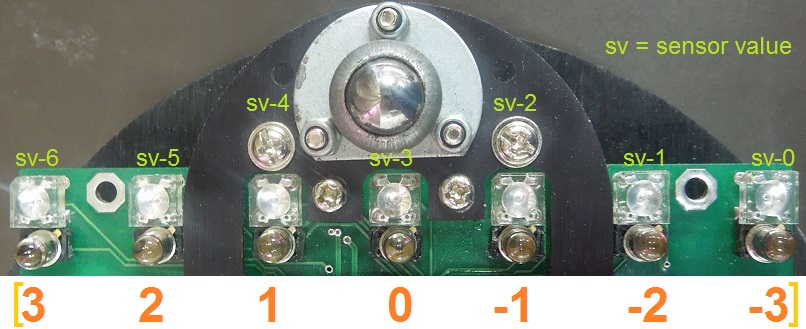
\includegraphics[scale = 0.4]{7-white-line-sensor-strip.png}
					\end{figure}
				\item Here the sensor values(sv) have to be manually or auto calibrated, so as to provide the symmetric values on both sides of the line to be followed.  
  			\end{itemize}
		\end{frame}

	\section{PID Implementation}
	\begin{frame}{PID Implementation}
		\begin{itemize}
			\item As shown in figure Final Sensor Value will be obtained after multipling values from matrix with the corresponding sensor value, i.e. \\
			SV = (-3)*(sv0) + (-2)*(sv1) + (-1)*(sv2) + 0*(sv3) + 1*(sv4) + 2*(sv5) + 3*(sv6) 
			\item For a white line follower all sensors which are on white line (mostly middle 2-3 sensors) will have different sensor values and all sensors which are on black/other line will have different sensor values.
			\item So variable SV will have different values as the bot moves left , right or forward/backward and will give deviation from SetPoint, i.e. error , which is input to PID Controller.
			\item For Example- If bot wobble towards left side of the white line, SV value provide negative values to the PID controller, and using those values PID Controller will control the left or right motor speed to align the bot on the white line, same case when bot wobble towards right of White Line.
			
		\end{itemize}
	\end{frame}

	\section{Basic Terminology}
		\begin{frame}{PID COntroller Basics}
		
			The basic terminology we use to implement the PID Controller are: 
		\begin{itemize}
			\item \textbf{Error(e):} The error is the amount by which robot is deviating from it’s set-point. 
			\item \textbf{Proportional(P):} The proportional component depends only on the difference between the set point and the process variable. This difference is referred to as the Error term. 
			\item \textbf{Integral(I):} The integral component sums the error term over time. 
			\item \textbf{Derivative(D):} The derivative component causes the output to decrease if the process variable is increasing rapidly. The derivative response is proportional to the rate of change of the process variable.	 
		\end{itemize}
	\end{frame}
	
	\section{PID Constant Factors}
	\begin{frame}{PID Constant Factors}
		\begin{itemize}
			\item Each term (P, I, D) will need to be tweaked in the code. Hence , they are included in the code by multiplying with respective constants.
			\item Proportional Constant(Kp): It is used to increase or decrease the impact of Proportional.
			\item Integral Constant(Ki): It is used to increase or decrease the impact of Integral.
			\item Derivative Constant(Kd): It is used to increase or decrease the impact of Derivative.
		\end{itemize}
	\end{frame}
	
	\section{Block Diagram of PID Controller}
		\begin{frame}{Block Diagram of PID}
			\begin{itemize}
			 \item Output obtained from PID Controller after processing on the error will be added or substracted in motor speed depending on the nature of output(i.e. positive or negative).
				\begin{figure}
				\centering
				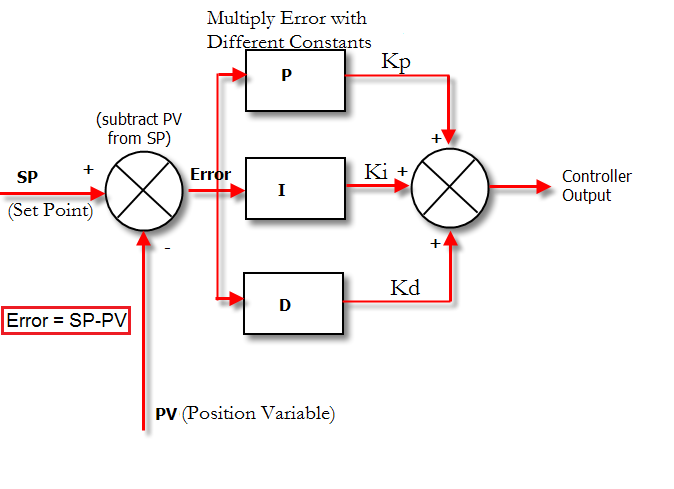
\includegraphics[scale = 0.5]{pid_simplified.png}
				\end{figure}
			\end{itemize}
		\end{frame}
	
	
		\section{PID Formula}
		\begin{frame}{PID Formula}
			\begin{itemize}
				\item Here we use PID Formula to calculate the Correction ,i.e. the output of PID Conrolleras follows: \\
					  Correction= proportional * Kp + integral * Ki + derivative *Kd	\\
					\text where  
					 \begin{enumerate}
					  \item error(e) = position $-$ setpoint \\
					  \item proportional(p) = proportional + error \\
					  \item integral(i) = integral + proportional	\\ 
					  \item derivative(d) = proportional $-$ last proportional	\\
					 \end{enumerate} 
			\end{itemize}
		\end{frame}
	
	\section{Parameter Comparision }
		\begin{frame}{Comparision}
			\begin{itemize}
				\item Summarizing PID Controller:-
				% \frametitle{Table}
				\begin{table}
				\begin{tabular}{||c| c| p{5 cm}||}
				%	\toprule
					\hline
					\textbf{term} & \textbf{constant} & \textbf{effect}\\
					\hline
				%	\midrule
					Proportional & Kp & It reduces a large part of error based on present error.
					 \\ \hline
					Integral & Ki & Cumulative of a small error would further help reduce the final error.
					 \\ \hline
					Derivative & Kd & Counteracts the Kp and Ki terms when the output changes quickly. \\
				%	\bottomrule
				\hline
				\end{tabular}
				% \caption{Table caption}
				\end{table}
			\end{itemize}
		\end{frame}
		
		
	\section{Waveform Characteristics for PID}
		\begin{frame}{Waveform Characteristics for PID} 
			\begin{itemize}
				\item Commonly, the response is quantified by measuring defined waveform characteristics between PID Paremeters and Time:
					\begin{figure}
						\centering
						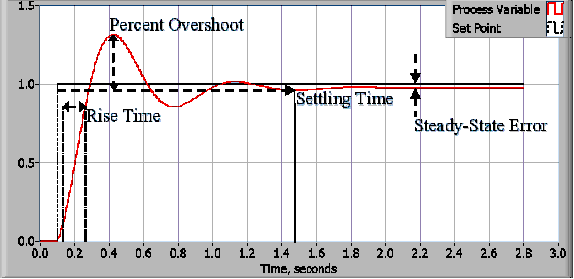
\includegraphics[scale = 0.5]{PID_Characteristic.png} \\
						%\text Fig. Characteristic Waveform of PID Controller
					\end{figure} 
				\item \textbf{Rise Time} is the amount of time the system takes 
				to go from 10 percent to 90 percent of the steady-state, or final value.
				\item \textbf{Percent Overshoot} is the amount 
				that the process variable overshoots the final value,
				expressed as a percentage of the final value.
			\end{itemize}	 
		\end{frame}
	
		\section{Waveform Characteristics for PID}
		\begin{frame}{Waveform Characteristics for PID} 
			\begin{itemize}
				\item \textbf{Settling time} is the time required for the process variable
				to settle to within a certain percentage (commonly 5 percent) of the final value.
				\item \textbf{Steady-State Error} is the final difference between the position variable(PV) and set point(SP).
				\item Effect of Increasing a Parameter Independently :-
				\begin{table}
					\begin{tabular}{||p{1 cm}|p{1.2 cm}|p{1.2 cm}|p{2 cm}|p{1.5 cm}||}
						%	\toprule
						\hline
						\textbf{Para- meter} & \textbf{Rise Time} & \textbf{Over shoot} & \textbf{Settling Time} & \textbf{Steady State Error} \\
						\hline
						%	\midrule
						\textbf{Kp} & Decrease & Increase & Small Change & Decrease \\
						\hline
						\textbf{Ki} & Decrease & Increase & Increase & Eliminate \\
						\hline
						\textbf{Kd} & Minor Change & Decrease & Decrease & No effect \\
						\hline
						%	\bottomrule
					\end{tabular}
					% \caption{Table caption}
				\end{table}
			\end{itemize}	 
		\end{frame}
	
	\section{Tuning}
		\begin{frame}{Tuning}
			\begin{itemize}
			\item PID implementation would prove to be useless rather more troublesome unless the constant values are tuned depending on the platform the robot is intended to run on.
			\item PID Tuning is difficult in most cases as there is no proper way to tune , other than experimentally.
			\item basic guidelines that will help reduce the tuning effort:
			\begin{itemize}
			\item \text Start with Kp, Ki and Kd equalling 0 and work with Kp first. Try setting Kp to a value of 1 and observe the robot. The goal is to get the robot to follow the line even if it is very wobbly. If the robot overshoots and loses the line, reduce the Kp value. If the robot cannot navigate a turn or seems sluggish, increase the Kp value.
			\item \text Once the robot is able to somewhat follow the line, assign a value of 1 to Kd (skip Ki for the moment). Try increasing this value until you see lesser amount of wobbling. 
			\end{itemize}
		\end{itemize}
	\end{frame}	
	
	
	\section{Tuning}
		\begin{frame}{Tuning}
			\begin{itemize}
		\item \text Once the robot is fairly stable at following the line, assign a value of 0.5 to 1.0 to Ki. If the Ki value is too high, the robot will jerk left and right quickly. If it is too low, you won't see any noticable difference.  Since Integral is cumulative, the Ki value has a significant impact. You may end up adjusting it by .01 increments. \\
		
		\item \text Once the robot is following the line with good accuracy, you can increase the speed and see if it still is able to follow the line. Speed affects the PID controller and will require retuning as the speed changes.
			\end{itemize}
		\end{frame}


	\section{Thank You}
	\begin{frame}{Thank You}
		\centering THANK YOU !!!
	\end{frame}

\end{document}



